\section{Introduction}
\par The modeling of motor-propeller dynamics in the context of multi-rotor vehicles takes various forms, ranging from idealized representations to more complex realities. These idealizations include modeling as input uncertainties \cite{yacef2016observer}, \cite{liang2021geometric}, \cite{wang2018backpropagating}, linear dynamics \cite{pounds2010modelling}, or stationary mappings \cite{tayebi2006attitude}. However, these models often oversimplify the polynomial nonlinearity inherent in actuator dynamics, which encompasses factors like friction and aerodynamics.

The rotational inertia and the substantial mass of large propeller blades
introduces time-scales comparable to those of the overall drone dynamics. These
dynamics play a pivotal role in achieving precise and controllable forces and
maneuvers \cite{hamandi2021design}. Such precision and control are of
paramount importance in the emerging field of aerial manipulation, where large
multi-rotors with diverse configurations are employed \cite{ding2021design},
\cite{ryll20176d}, \cite{jiang2017estimation}.

While open-loop control simplifies actuator design, it has limited
effectiveness in increasing bandwidth \cite{charla2022enhancing} and can
amplify uncertainties. Therefore, feedback mechanisms, such as monitoring
actuator inputs for calculating aerodynamic power \cite{B_Manony} or propeller
RPM \cite{franchi2017adaptive}, \cite{bangura2017thrust}, become necessary.
However, note that the former methods may suffer from calibration errors. The
proliferation of commercially available BLDC RPM sensors, designed to transmit
commutation signals, now enables reliable RPM measurements in medium-sized
drones.

The earlier studies that employed RPM feedback to enhance system dynamics, such
as \cite{pounds2009design},\cite{pounds2007system},\cite{mahony2012multirotor}
relied on a second-order model around hover conditions. This approach, while
effective for minor input variations, may not be suitable for accommodating
substantial input changes. In contrast, \cite{franchi2017adaptive} implemented
a hybrid controller using RPM feedback to linearize actuator dynamics. However,
this method necessitates low-level access to the Electronic Speed Controller
(ESC) microcontroller. A notable challenge when using commercial Electronic
Speed Controllers (ESCs) designed for manual control in autonomous operations
is their thrust-to-input curve is linearized \cite{Phang} for intuitive
operability. Usually, this is achieved by introducing nonlinear compensation in
the seed controller of the ESC and the actual PWM input to the inverter
controlling the BLDC motor (Fig.-\ref{fig::bldc_diag}). However, attempting to
estimate this compensation through system identification techniques proved to
be unfeasible.
%===
\begin{figure}[h]
    \centering
    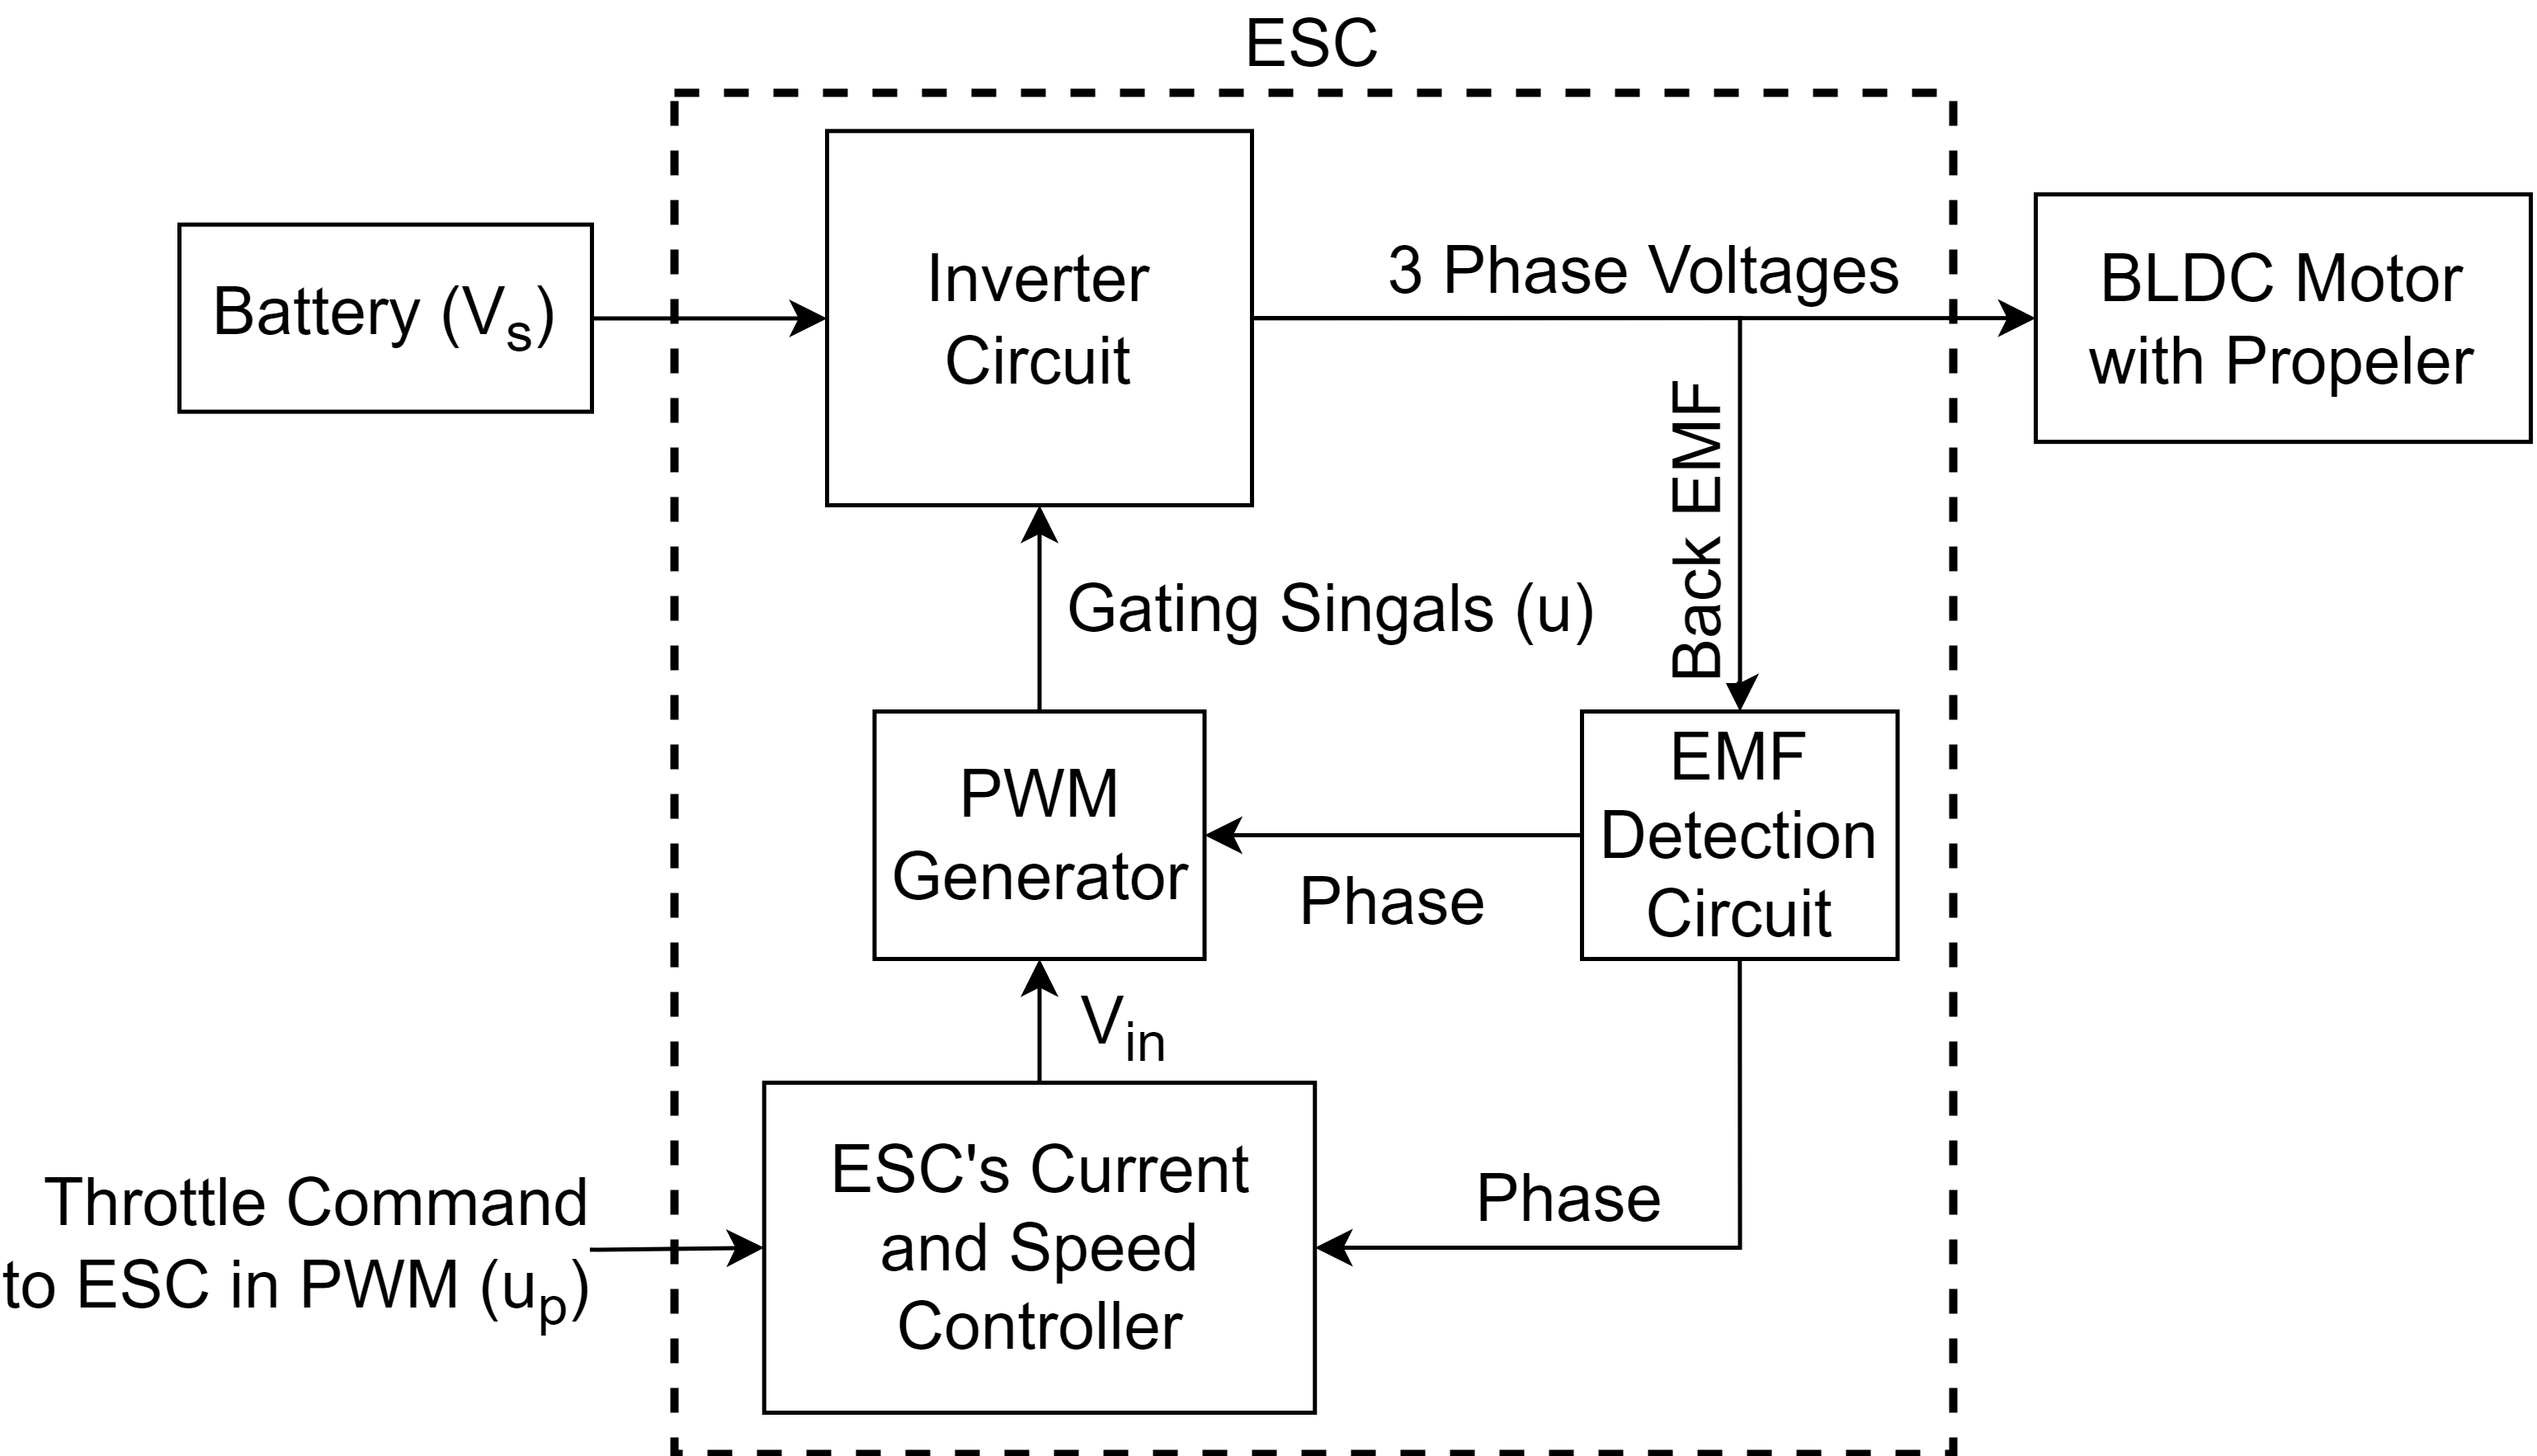
\includegraphics[width = \figsize]{./figs/figs_acc/schematic/esc_schematic.png}
    \caption{Schematic of ESC with BLDC motor}
    \label{fig::bldc_diag}
\end{figure}
%===

The present work introduces an adaptable input definition ($u_\omega$) capable of accommodating any nonlinear compensatory mechanisms within the ESC that define ($u_p$). Utilizing this input definition, the nonlinear control model of the system is developed. This model enables the design of improved controllers capable of explicitly mitigating uncertainties stemming from the model parameter uncertainties, whose bounds are estimated experimentally. Additionally, a novel RPM measurement algorithm with high, variable resolution was discussed, deviating from conventional constant resolution approaches. Furthermore, the paper outlines a system identification procedure linking the linearized model parameters to the parameters of a full nonlinear model.

The paper is structured into five main sections. Following this introduction,
Section-2 delves into the discussion of the experimental setup and the
measurement algorithm. In Section-3, we provide a comprehensive overview of the
full nonlinear dynamic model, introduce the normalized angular velocity input
definition, and establish the small perturbation model based on these
foundations. Section-4 encompasses model parameter identification and validation
results. Finally, Section-5 offers concluding remarks.
